\documentclass[10pt,twocolumn]{article}

% use the oxycomps style file
\usepackage{oxycomps}

% read references.bib for the bibtex data
\bibliography{references}

% include metadata in the generated pdf file
\pdfinfo{
    /Title (Comps Proposal)
    /Author (Roberto Villegas Jr)
}

% set the title and author information
\title{Comps Proposal}
\author{Roberto Villegas Jr.}
\affiliation{Occidental College}
\email{rvillegas@oxy.edu}

\begin{document}

\maketitle

\section{Introduction and Problem Context} % What is LoL? Personal importance? Relevant information needed to understand the problem?

For my project, I will make a League of Legends (LoL) Esports information web application.
League of Legends is a MOBA video game played on PC, and is considered one of the most popular video games in the world.
As a result, professional LoL leagues around the world are some of the most popular Esports leagues in the world, with viewership peaking at 200k every week for the top LoL leagues.
Fans, like in any other traditional sport, make a hobby of keeping up with teams in their region and watching the games every weekend.
It is common to see fans comparing team statistics and standings with each other on online forums, as well as specific team forums with fans sharing opinions about players (sometimes good, sometimes bad). 
Fans also often look up to the players to learn how to improve their own skill in the game, watching them to see who the strongest champions (characters in the game) are and what game items are the best.
The problem with this is that there aren't many places you can easily look this information up.
Much of it is scattered around the internet, and it takes time to find the exact information you are looking for.

My web application will be a one-stop shop for all of this information relating to LoL Esports, including match information, team and player history, and a player's LoL status.
Match information is any information about what has happened in a match.
This includes in game statistics like a player's Kill/Death/Assist ratio (KDA), a player's item build, a team's record and match history, and more.
I also want to include live match information as a game is happening.
This information would include things that are not shown (or not consistently shown) on the livestream of the match, including a player's gold (the game's currency) amount, total damage, and more.
My goal is for this to be an extra source of match information while the user is watching the livestream, rather than something you can have if you cannot watch the game live.

Team and player history will include information like past players, current standings, and team accomplishments for teams, as well as past teams, career statistics, and past teams for players.
This is more comparable to a biography of players and organizations involved with LoL Esports, though I would like to include more technical information involving LoL.

A player's LoL status refers to if a pro player is playing LoL on their personal account.
"Tracking the pros" would be made easier with my web application, as it will tell you if/when a player is in a match, as well as give you the opportunity to watch their match live with LoL's built-in spectator mode.
There will also be a history of a player's past matches and their statistics so fans can see what a player has been experimenting with.

\section{Technical Background} % Language? Framework? What is your approach?
I have chosen (for now) to work on this project using the Django web framework.
I based this decision on the fact that this will be a relatively quick project (about 6 months total) and my own familiarity with Python.
It will be my first time using Django, as well as building a web app in general, so there will need to be a dedicated time for me to learn everything before the project fully starts (more on this later).

This project will run on the use of 3 different sources of information through APIs.
The web application will pull all the information from these sources and display them for the user to see and interact with.
Some information will be straightforward and not require much programming between the sources and the application.
For example, a player's team history may be an array of strings for team names, which I will use to display onto the application.

Other information is much less straightforward and will require lots of code to work properly on my application.
For example, to properly track pro players playing LoL outside of the pro leagues, I will need to first locate a list of the player's known game IDs (some players have hidden accounts to prevent harassment in the game).
Then, we will feed these IDs through an API to see who is current playing the game, and if so, what their live stats are.
Once we have this, we still need to figure out how to display this information as it is being updated in real time.
The challenge with this is figuring out how to share this information without a long delay between the game and my application.
LoL's built-in spectator has a 3 minute delay coded into it to prevent cheating and maintain competitive integrity, so I want to aim to keep the delay of the entire process around 3 minutes total.

Live information about a pro match currently happening is also another challenge I will face.
Currently, I don't have a source for this information.
I know there are ways to access information, as there is a Twitter account (@LoLEsportsStats) that shares game information before and after a game occurs.
The problem with this is that the account is run by Data Scientists and Statistic Operators for their respective leagues, so this information may not be available for public use.

\section{Prior Work} % Strafe App
There exists a phone app that tracks Esports leagues called Strafe, which is comparable to an ESPN app for Esports.
It covers about 10 different games and their professional leagues, from Counter Strike to Valorant.
It allows users to set their favorite games and teams and provides notifications whenever any matches occur, news breaks, or general updates.
It also provides basic information, such as a league's schedule and standings.

The app is great if you need something to keep track of your favorite teams on the go.
However, it doesn't provide the specific details I want to look for.
Perhaps this is because it has to cover multiple different games at once other than just LoL, but the app lacks specific details about matches that LoL Esports fans would find even more interesting.

\section{Methods}

There is plenty of things needed to be done in order to get this project in full swing.
Since I am at a disadvantage with experience in making a web application, a chunk of my time will be spent learning about how to use the Django framework.
This includes finding online resources about Django and creating my own test project to know how everything works.
Django's online documentation includes a tutorial on how to create a simple project using Django, which I expect to use to familiarize myself.

The development of the web app begins with a brainstorm of how the project and all of its components will work together to become the final project.
A better understanding of this will come after I learn about Django, databases, and APIs much later, but for now I know that the web app consists of three main parts: the front end, the back end, and the database.
Throughout the end of the summer and the beginning of the semester (the first 3-5 weeks), the database will be coded to organize information from the projects multiple sources and send this organized information to the back end.
I am not sure if it is possible for the database to be used both ways (sources-to-database, database-to-project backend) in a single back end, so this issue must be resolved early in the project's development.
Development of the front end will be left to be done closer to this project's deadline.
Not to say that the front end is not important at all, but making sure the back end and the database can reliably work is arguably the most important issue of the project.
Failure by either one of these sections will cause the entire web app to not work as intended.

\section{Evaluation Metrics}

Luckily, the LoL Esports season will still be in progress during the development of this project.
This means that there is an environment with consistent changes and tests to evaluate the performance of the project.
The most common data changes during this time include match history, league/tournament standings, roster changes, and much more.

The most important quality the project should focus on is its speed.
Like any other sports fan, LoL Esports fans like to know when something happens as soon as it happens.
Any delay in the data being added to the database and updating the front end of the web app means failure in the project.
Thus, the web app's speed must be tested to ensure the reliability of the information being shown and thus the reliability of the entire project.

Speed is not only important for how the information gets to the user from the source, but also how quickly the information can load.
This is more of an issue with how everything is developed, but it can still be considered an important metric when evaluating a web app.
There is likely going to be plenty of information available at a single click, so the web app must be prepared to move this information through the back and front ends ina timely manner.
Failure of this also means a failure of the entire project.

\section{Ethical Considerations}

\subsection{Accessibility}

The largest and most important ethical concern about the project is its accessibility.
Since the purpose of the project is to display information to users, the project's priority must be to consider how different people digest information.
This has less to do with a user's preferences and more to do with a user's ability to digest information.
For example, a user with "perfect" vision can easily read a web page with information while a blind user won't know anything about the web page unless it includes and incorporates audio features.
Even a user's access to technology must be considered, requiring the project to be accessible to multiples devices instead of only one.
The three different areas of accessibility the project must pay attention to are visually impaired user, users with physical disabilities, and device limitations.

\subsubsection{Visually Impaired Users}

It is obvious how a visually impaired user will have trouble using web app like this one, especially if there were no features to enable their accessibility.
It is important to note that there are more than just blindness; colorblindness, partial blindness, and much more are things that need to be considered in order to make the web app truly accessible for anyone with a visual impairment.

The American Foundation for the Blind's (AFB for short) website lists plenty of tips to help web developers make their websites more accessible for those with visual impairments \cite{AFBAccessibilityResources}.
First, making a website keyboard accessible will make it plenty easier for these users to navigate through the website \footnote{\url{https://www.afb.org/consulting/afb-accessibility-resources/keyboard-accessibility}}.
Keyboard navigation is the "traditional" approach to website for visually impaired users, so designing the website with keyboard tools in mind is important.
For example, one should be mindful about the design of the Document Object Model for the website, since screen readers will rely on this to read the website contents in the order that they appear in the DOM.
Failure to properly order its contents can make information on the website confusing for the user.
Additionally, the AFB suggests to use native HTML controls in order since these are an "established standard". Attempting to use different controls might make it more difficult to differentiate parts of the website and overcomplicate website navigation.

The AFB also outlines how effective image and video descriptions can be in a website.
Since a user's tools won't be able to "read" an image or video, additional text is required for the reader to figure out what is being shown.
For images, this is done in the form of alternative (alt for short) text \footnote{\url{https://www.afb.org/consulting/afb-accessibility-resources/improving-your-web-site}}.
These texts are brief and highlight important information about what the image is showing.
Putting essential information and context into an alt text makes the difference between a good and bad alt text.
For example, an alt text that says "business man in a suit" does not have the same effect as "Bill Gates, co-founder of Microsoft".
For videos, the inclusion of "audio description" fulfills the same purpose \footnote{\url{https://www.afb.org/consulting/afb-accessibility-resources/video-description}}.
% more about audio description if I have time

Lastly, the colors used by the website matters to those with impairments affected by color (such as those with colorblindness).
Using colors without much contrast can make it hard to make out what a website is saying, or figure out where different buttons or other tools are.
Color choice is important when making a website, and can open the website up to more people who want to use it.

\subsubsection{Users with Physical Disabilities}

The project should also consider users that may physically struggle to navigate it.
Alternative devices designed for the physically disabled already exist, such as things like modified keyboard (fewer keys, larger keys, etc.) and Lomak keyboards (light-activated device mounted on a user's head, see Figure \ref{fig:LomakKeyboard}).
Still, a responsible and ethical programmer will make sure to still include web app features to ensure that everyone has equal access and use to the project.

\begin{figure}[ht!]
    \centering
    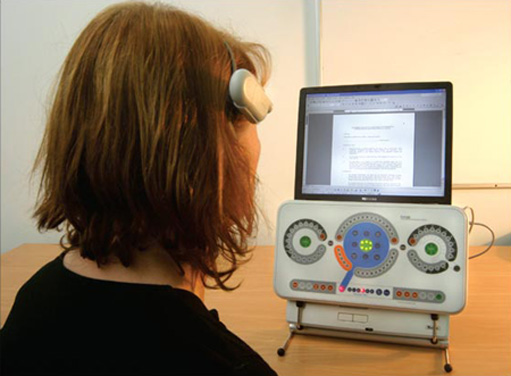
\includegraphics[width=.95\linewidth]{LomakKeyboard.jpg}
    \caption{
        Lomak Keyboard in use.
    }
    \label{fig:LomakKeyboard}
\end{figure}

% Links unable to be added due to error
The Web Content Accessibility Guidelines (WCAG for short) outlines how developers can make their web product more accommodating for those with disabilities, including physical disabilities \cite{WCAG2point1}.
For example, there is a guideline that explains how pointer cancellation should work with a single-pointer operation of a web app. % Link 1: https://www.w3.org/TR/WCAG21/#pointer-cancellation
This is specifically to help those that might input something they don't intend on inputting, and allowing them to continue viewing whatever page they're on instead of changing pages and struggling to get back to where they were.
There is also a guideline that sets a minimum "target size" for page elements so that things are not too small and impossible to click on. % Link 2: https://www.w3.org/TR/WCAG21/#target-size

Additional adjustments can be done by creating a separate layout aimed at helping users with physical disabilities. The main action of this feature would be to create bigger buttons and use the previously mentioned guidelines so that users will be able to click on buttons and navigate through the page without much struggle. 

\subsection{Privacy}

These days, one of the biggest concerns for users is their privacy.
Any and all data collected and stored by any software must be held ethically and with the express consent of the user.
The current plans of this project include an "account" system that allows users to create an account with their favorite preferences such as favorite teams, players, leagues, etc.
It will also have the capability of sending notifications to the user either through email or (possibly) text, which is where the focus for privacy comes in.

To give users control of their private information, an email or phone number will not be required when making an account.
The notification feature will be entirely optional, and any user that only wants to access the information in the web app from time to time will be able to do so privately.
Additionally, a user can use this web app without making an account, essentially allowing anonymous users.

\subsection{Security}

Although there is not a significant amount of sensitive information that must be protected in this project, a good security system is still required so that a user's information does not get use improperly or maliciously.
Handling a user's information with care is a responsibility of a developer, and this project is no exception.

Firstly, usernames and passwords must be stored and transported securely.
This means making sure this information is encrypted from the user's end as well as in the database.
A simple hash function somewhere in between the front end and the back end should be able to provide some security for this.
This will also help with email addresses and phone numbers.

\section{Timeline}

\printbibliography

\end{document}
